% Gemini theme
% https://github.com/anishathalye/gemini

\documentclass[final]{beamer}

% ====================
% Packages
% ====================

\usepackage[T1]{fontenc}
\usepackage{lmodern}
\usepackage[size=custom,width=121.92,height=91.44,scale=1.5]{beamerposter}
\usetheme{gemini}
\usecolortheme{isu}
\usepackage{graphicx}
\usepackage{booktabs}
\usepackage{tikz}
\usepackage{pgfplots}
\usepackage{minted}
\usepackage{qrcode}

\usemintedstyle{lovelace}
\setminted{autogobble=true}

% ====================
% Lengths
% ====================

% If you have N columns, choose \sepwidth and \colwidth such that
% (N+1)*\sepwidth + N*\colwidth = \paperwidth
\newlength{\sepwidth}
\newlength{\colwidth}
\setlength{\sepwidth}{0.025\paperwidth}
\setlength{\colwidth}{0.3\paperwidth}

\newcommand{\separatorcolumn}{\begin{column}{\sepwidth}\end{column}}

% ====================
% Title
% ====================

\title{Cross Section Analysis in MetPy}

\author{Jonathan E. Thielen \inst{1} \and Ryan M. May \inst{2} \and John R. Leeman \inst{2}}

\institute[shortinst]{\inst{1} Department of Geological and Atmospheric Sciences, Iowa State University, Ames, IA \samelineand \inst{2} Unidata/UCAR, Boulder, CO}

% ====================
% Body
% ====================

\begin{document}

\begin{frame}[t, fragile]
\begin{columns}[t]
\separatorcolumn

\begin{column}{\colwidth}

  \begin{block}{Background}

    \begin{itemize}
      \item Cross sections are a common meteorological plot, often used in analysis of:
        \begin{itemize}
          \item Convective systems
          \item Isentropic ascent
          \item Tropopause folds
          \item Conditional Symmetric Instability (CSI)
        \end{itemize}
      \item The General Meteorology Package (GEMPAK) has the ability to obtain and plot such vertical cross sections through three-dimensional data, however, this functionality has been lacking until recently in MetPy. 
        \begin{figure}
          \centering
          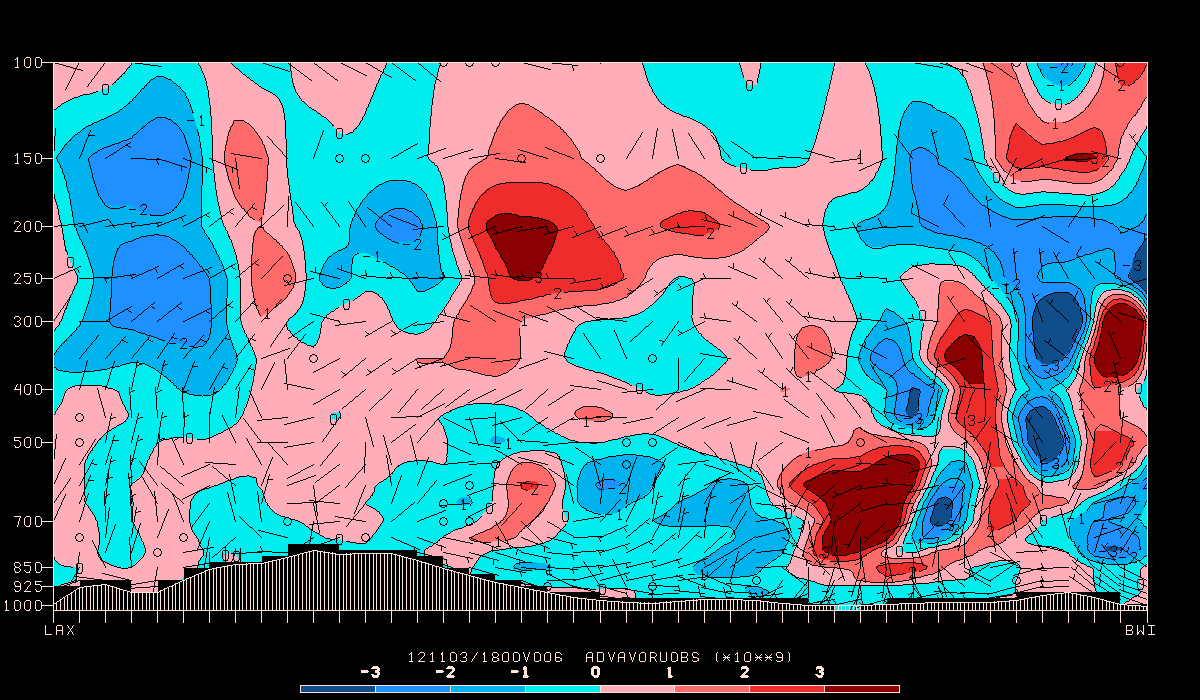
\includegraphics[height=4.5in]{figures/gempak_cross.png}
        \end{figure}
      \item Cross section interpolation (utilizing xarray) is now included in MetPy based on work undertaken during the 2018 Unidata Summer Internship.
    \end{itemize}

  \end{block}

  \begin{alertblock}{xarray and MetPy}

    xarray is a powerful Python package that provides N-dimensional labeled arrays and datasets following the Common Data Model with many useful utility methods for indexing, interpolating, and reducing data. MetPy is transitioning to using xarray as its primary data model and includes of number of helper methods via an accessor interface, such as those below:

    \begin{minted}{python}
      import xarray as xr
      from metpy.units import units

      # Parse for CRS and coordinate types
      data = xr.open_dataset('data.nc').metpy.parse_cf()

      # Get a Cartopy CRS
      data['temperature'].metpy.cartopy_crs

      # Unit and coordinate helpers
      data['temperature'].metpy.sel(
          vertical=500 * units.hPa)
      data['u_wind'].metpy.convert_units('knots')
    \end{minted}

  \end{alertblock}

\end{column}

\separatorcolumn

\begin{column}{\colwidth}

  \begin{exampleblock}

    \vspace{-1.5em}

    \begin{figure}
      \centering
      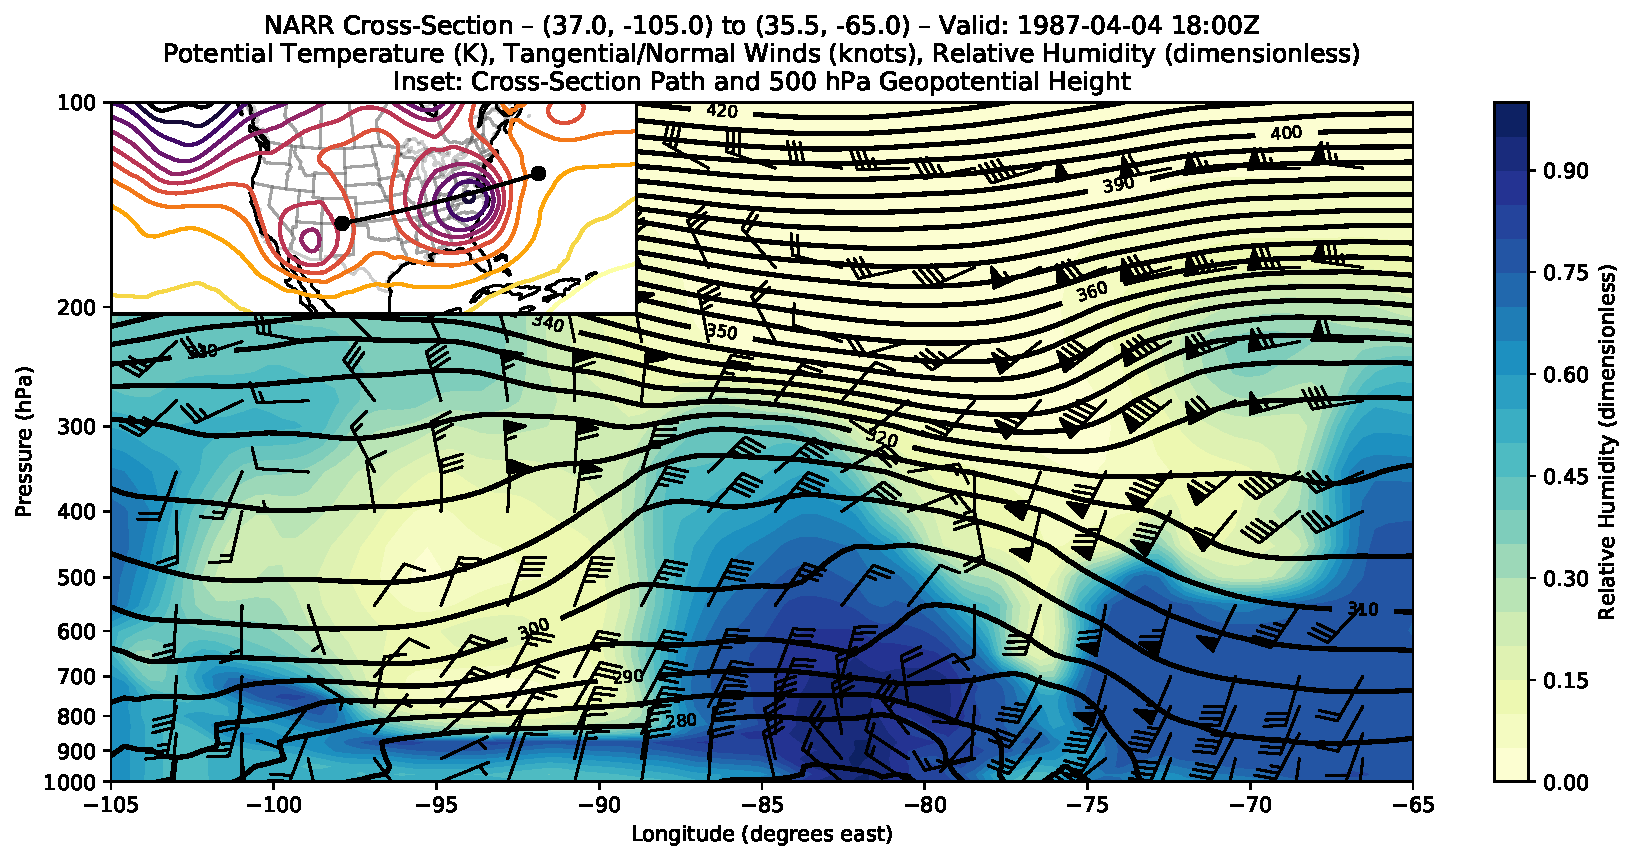
\includegraphics[width=\colwidth]{figures/basic_example_narr.pdf}
      \caption{Basic cross section example using NARR data, with demonstration of wind components (included in MetPy documentation).}
    \end{figure}
    \begin{figure}
      \centering
      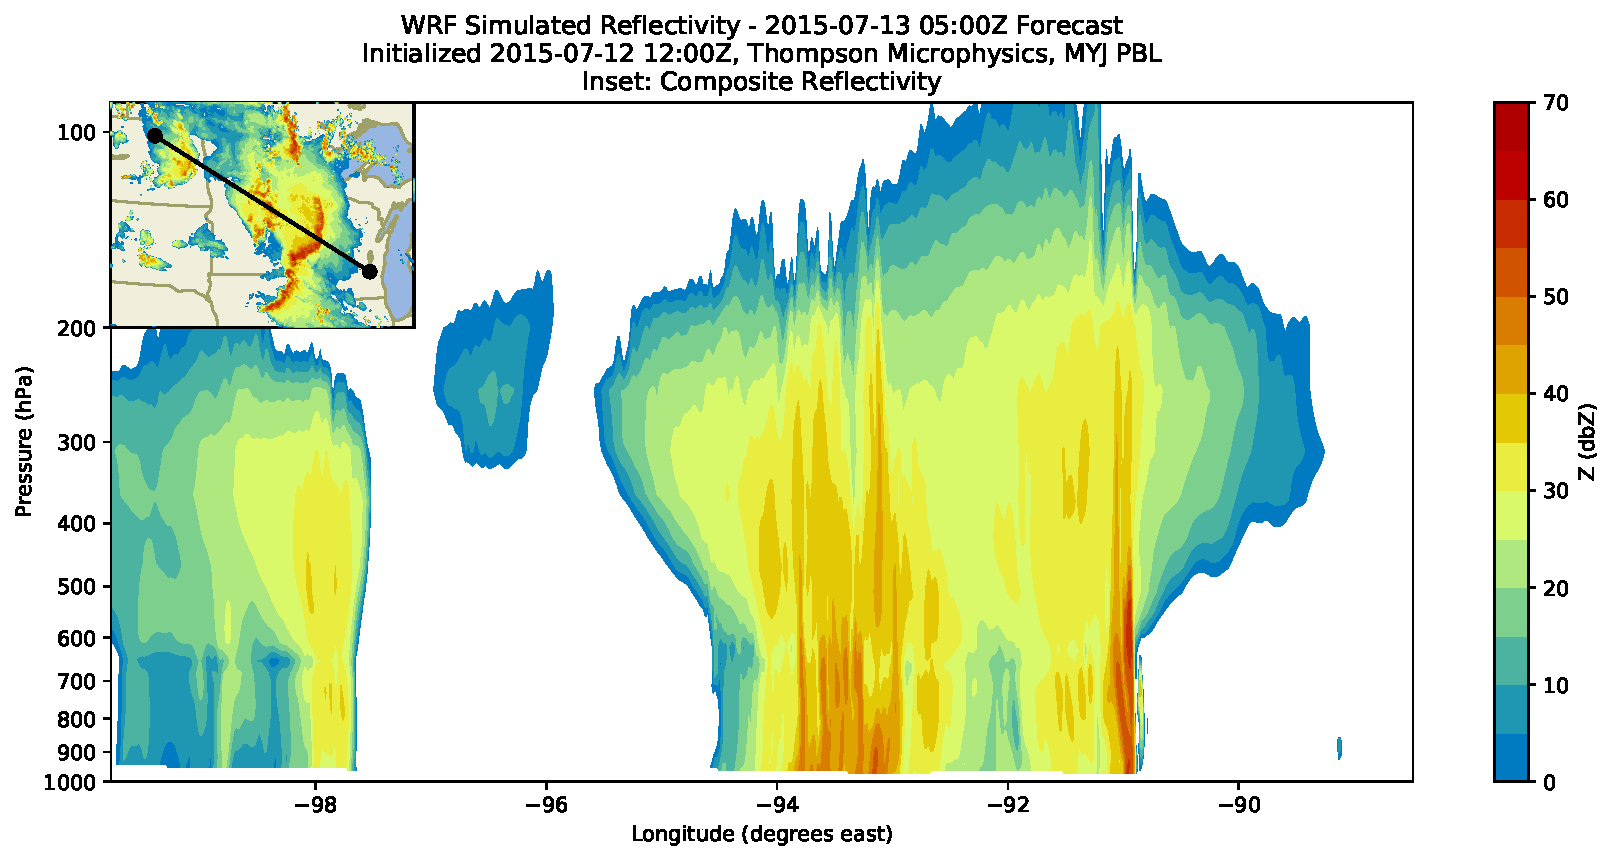
\includegraphics[width=\colwidth]{figures/wrf_refl.pdf}
      \caption{Cross section of simulated reflectivity through a bow echo as simulated in a 1-km WRF-ARW run.}
    \end{figure}
    \begin{figure}
      \centering
      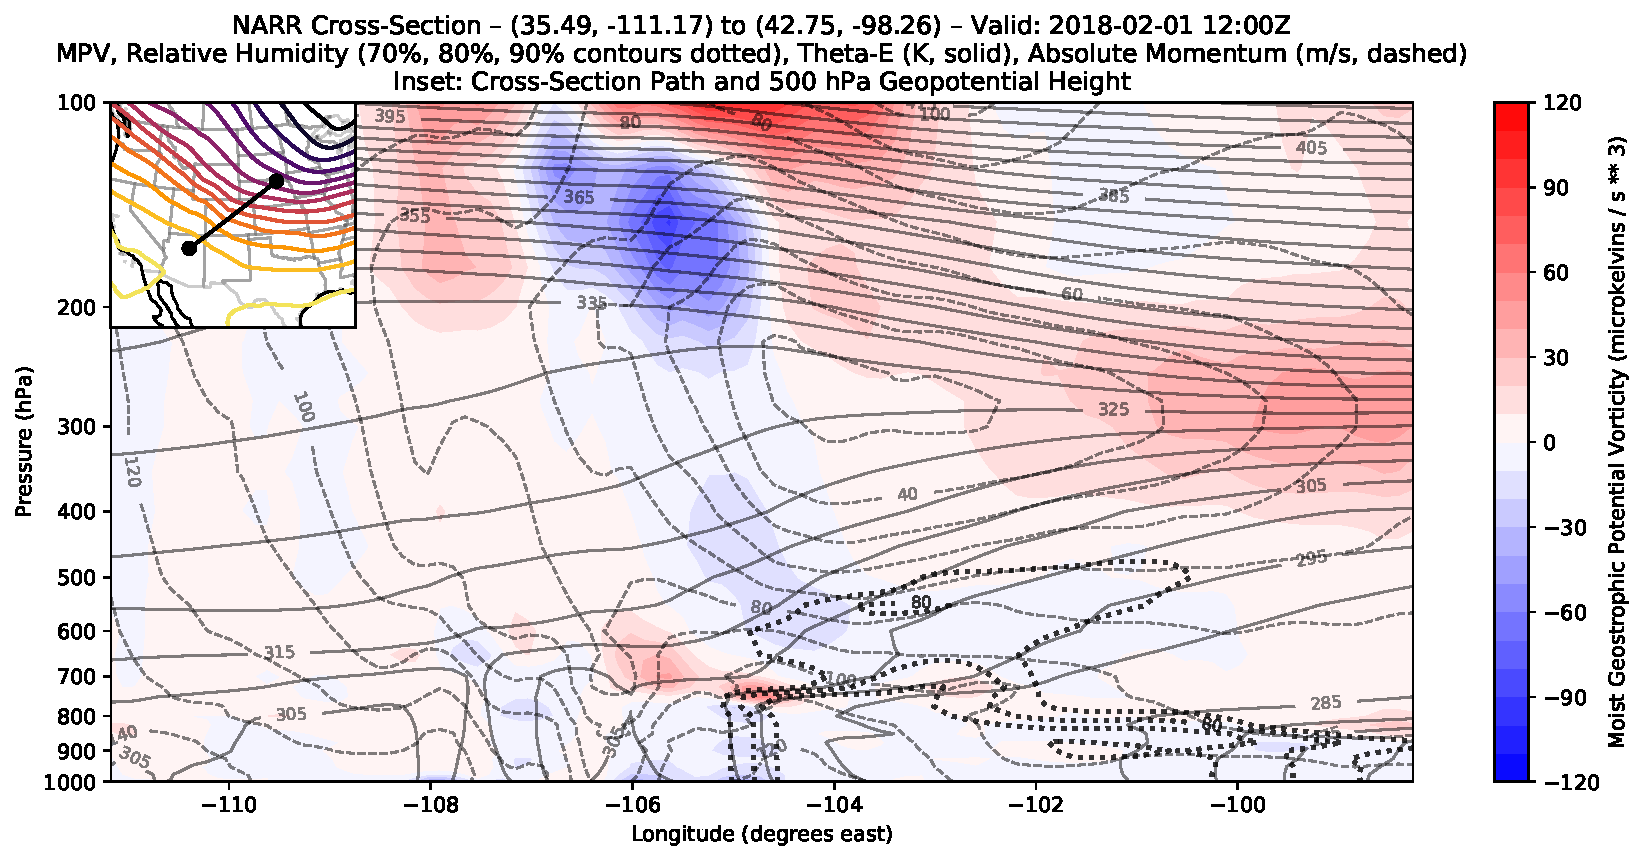
\includegraphics[width=\colwidth]{figures/csi_example_narr.pdf}
      \caption{Cross section of Moist Potential Vorticity (MPV) and Absolute Momentum for assessing CSI.}
    \end{figure}

  \end{exampleblock}

\end{column}

\separatorcolumn

\begin{column}{\colwidth}

  \begin{block}{Implementation}

    \begin{itemize}
      \item Preliminaries with xarray integration
        \begin{itemize}
          \item Construction of Cartopy CRS from CF metadata and basic unit helpers (already implemented in v0.8)
          \item Systematic identification of coordinate types (from CF metadata, or regular expression parsing as a fallback) to automatically recognize which coordinate corresponds to the x, y, and vertical directions
          \item Derivative calculations updated to accept and return xarray DataArrays (while being coordinate-aware)
        \end{itemize}
      \item MetPy's \mintinline{python}{cross_section()} is currently a coordinate-type- and projection-aware wrapper for xarray interpolation
        \begin{itemize}
          \item Takes a number of steps and a start and end point as arguments, and constructs a geodesic path along which to interpolate the input gridded data
          \item Linear and nearest neighbor interpolation methods available
          \item Input gridded data must be at least three-dimensional (x, y, and vertical), and any extra dimensions (such as time or ensemble member) are preserved
          \item \mintinline{python}{interpolate_to_slice()} available for cross sections on arbitrary paths
        \end{itemize}
      \item Cross section calculations (such as projected wind components and cross-sectional absolute (or ``pseudoangular'') momentum) are also available
    \end{itemize}

  \end{block}

  \begin{block}{Future Work}

    \begin{itemize}
      \item Extending cross section interpolation to unstructured data, such as observed soundings
        \begin{itemize}
          \item Use MetPy's interpolation methods like Cressman, Natural Neighbor, and Radial Basis Function
          \item Needs easy way to access surface and upper-air observations and a reliable format to store metadata-rich unstructured data in xarray
        \end{itemize}
      \item Making these cross section plots easier using a declarative interface (see Talk 4.1 by Ryan May, ``Bringing GEMPAK-like Syntax to Python with MetPy's Declarative Plotting Interface'')
    \end{itemize}

  \end{block}

  \begin{exampleblock}

    Interested in finding out more or exploring some demo notebooks? Check out

    \vspace{1em} 

    \begin{figure}
      \centering
      \large{\url{https://github.com/jthielen/}\\ \url{metpy_cross_section_ams_2019}}

      \vspace{1em}

      \qrcode[height=3in]{https://github.com/jthielen/metpy_cross_section_ams_2019}
    \end{figure}

  \end{exampleblock}

\end{column}

\separatorcolumn
\end{columns}
\end{frame}

\end{document}
